
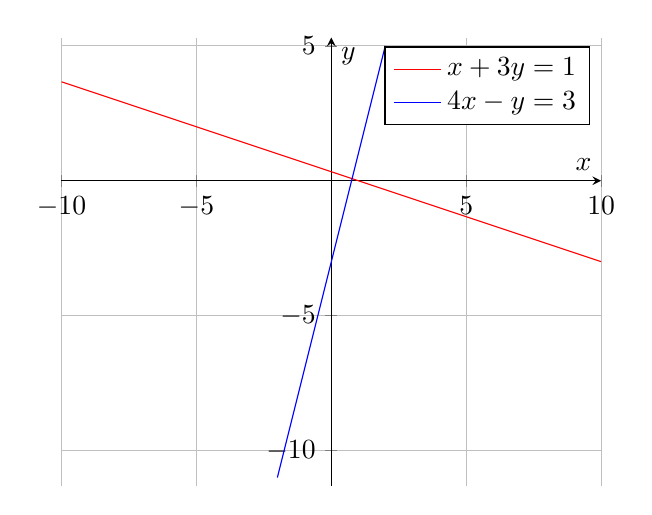
\begin{tikzpicture}[label distance=2mm]
\begin{axis}[
    axis lines = middle, axis equal,grid=both,
    xlabel = \(x\),
    ylabel = \(y\),
]
%Below the red parabola is defined
\addplot [
    domain=-10:10,
    samples=10,
    color=red,
]
{(x-1)/-3};

\addlegendentry{\(x + 3y = 1\)}
\addplot [
    domain=-2:2,
    samples=10,
    color=blue,
    ]
    {(4*x) - 3};
\addlegendentry{\(4x - y = 3\)}
\end{axis}
\end{tikzpicture}
